\documentclass[11pt]{article}
\usepackage[margin=1in]{geometry}
\usepackage{sectsty}

\usepackage{tabularx}
\usepackage{colortbl}
\usepackage{hhline}

\usepackage{amsmath}
\usepackage{algorithm}
\usepackage{algpseudocode}
\usepackage{float}   
\usepackage{amssymb}
\usepackage{amsmath}
\usepackage[pdftex]{graphicx}
\usepackage{subfig}
\usepackage[shortlabels]{enumitem}
\begin{document}
	\title{Machine Learning - Assignment 1}
	\author{\begin{small}--- Shikhar Vashishth\end{small}}
	\date{}
	\maketitle
	
	\subsectionfont{}
	\setlist[enumerate]{noitemsep}
	
\begin{flushleft}
		
\subsection*{Problem-1:}
$P(X)$ is defined as:
$$P(X=x1) = 0.1 + 0.1 = 0.2$$
$$P(X=x2) = 0.2 + 0.2 = 0.4$$
$$P(X=x3) = 0.1 + 0.3 = 0.4$$

$P(Y)$ is defined as:
$$P(Y=y1) = 0.1 + 0.2 + 0.1 = 0.4$$
$$P(Y=y2) = 0.1 + 0.2 + 0.3 = 0.6$$

$P(X|Y)$ is defined as:
$$P(X|Y) = \frac{P(X,Y)}{P(Y)}$$
$$P(X=x1|Y=y1) = 0.1/0.4 = 1/4$$
$$P(X=x2|Y=y1) = 0.2/0.4 = 1/2$$
$$P(X=x3|Y=y1) = 0.1/0.4 = 1/4$$
$$P(X=x1|Y=y2) = 0.1/0.6 = 1/6$$
$$P(X=x2|Y=y2) = 0.2/0.6 = 1/3$$
$$P(X=x3|Y=y2) = 0.3/0.6 = 1/2$$

$P(Y|X)$ is defined as:
$$P(Y|X) = \frac{P(X,Y)}{P(X)}$$

$$P(Y=y1|X=x1) = 0.1/0.2 = 1/2$$
$$P(Y=y2|X=x1) = 0.1/0.2 = 1/2$$
$$P(Y=y1|X=x2) = 0.2/0.4 = 1/2$$
$$P(Y=y2|X=x2) = 0.2/0.6 = 1/3$$
$$P(Y=y1|X=x3) = 0.1/0.4 = 1/4$$
$$P(Y=y2|X=x3) = 0.3/0.4 = 3/4$$

\subsection*{Problem-4:}
\subsubsection*{Part (a):}
\begin{figure}[H]
	\centering
	\fbox{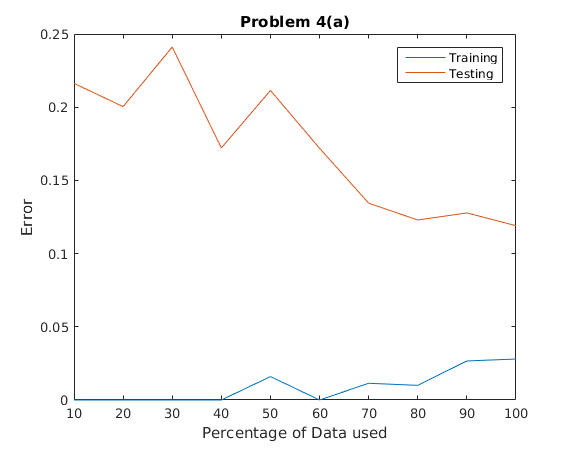
\includegraphics[scale=0.7]{../hw1_code_data/Problem4/plots/part-a/plot_4a.png}}
\end{figure}

\subsubsection*{Part (b):}

\begin{figure}[H]
	\centering
	\fbox{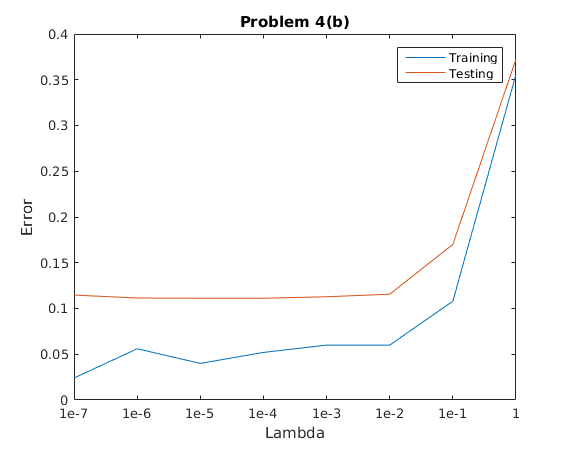
\includegraphics[scale=0.7]{../hw1_code_data/Problem4/plots/part-b/plot_4b.png}}
\end{figure}

\begin{center}
	\begin{tabular}{||c c c||} 
		\hline
		$\lambda$ & Training Error & Test Error \\ [0.5ex] 
		\hline\hline
		1.0e-07 & 0.0240 & 0.1147 \\
		\hline
		1.0e-06 & 0.0560 & 0.1115 \\
		\hline
		\textbf{1.0e-05} & \textbf{0.0400} & \textbf{0.1112} \\
		\hline
		0.0001 & 0.0520 & 0.1112 \\
		\hline
		0.0010 & 0.0600 & 0.1128 \\
		\hline
		0.0100 & 0.0600 & 0.1156 \\
		\hline
		0.1000 & 0.1080 & 0.1701 \\
		\hline
		1 & 0.3560 & 0.3726 \\
		\hline
	\end{tabular}
\end{center}

\begin{figure}[H]
	\centering
	\fbox{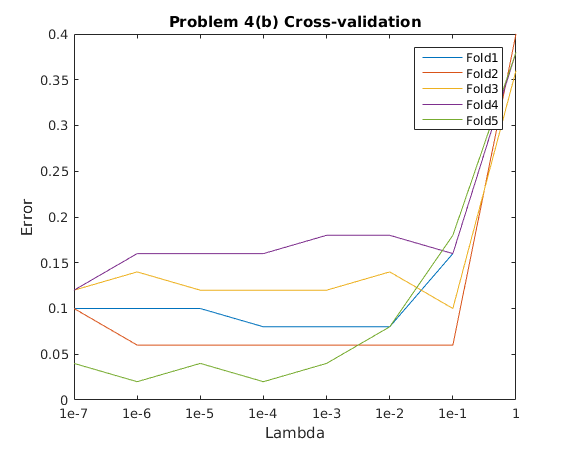
\includegraphics[scale=0.7]{../hw1_code_data/Problem4/plots/part-b/plot_4b2.png}}
\end{figure}

\textbf{Cross-validation:}
\begin{center}
	\begin{tabular}{||c c c||} 
		\hline
		$\lambda$ & Avg Training Error & Avg Test Error \\ [0.5ex] 
		\hline\hline
		\textbf{1.0e-07} & \textbf{0.0240} &\textbf{ 0.0240} \\
		\hline
		1.0e-06 & 0.0400 & 0.0400 \\
		\hline
		1.0e-05 & 0.0380 & 0.0380 \\
		\hline
		0.0001 & 0.0460 & 0.0460 \\
		\hline
		0.0010 & 0.0510 & 0.0510 \\
		\hline
		0.0100 & 0.0600 & 0.0600 \\
		\hline
		0.1000 & 0.1160 & 0.1160 \\
		\hline
		1 & 0.3730 & 0.3730 \\
		\hline
	\end{tabular}
\end{center}

The cross-validation method gave us a different value of $\lambda$ as $1.0e-07$ which is different from the $\lambda$ value which we got before. The cross validation process doesn't select the right value of $\lambda$.

\pagebreak
\subsection*{Problem-5:}

\subsubsection*{Part (a):}
Training Accuracy: \textbf{99.75} \\ 
Testing Accuracy:  \textbf{75.67}

\begin{table}[h!]
	\centering
	\caption{Confusion Matrix}
	\begin{tabular}{l|c|r}
		  & $\hat{y} =+1$ & $\hat{y} =+1$\\
		\hline
		$y =+1$ & 118 & 33\\
		$y =-1$ & 40 & 109\\
	\end{tabular}
\end{table}




\subsubsection*{Part (b):}

\begin{figure}[H]
	\centering
	\fbox{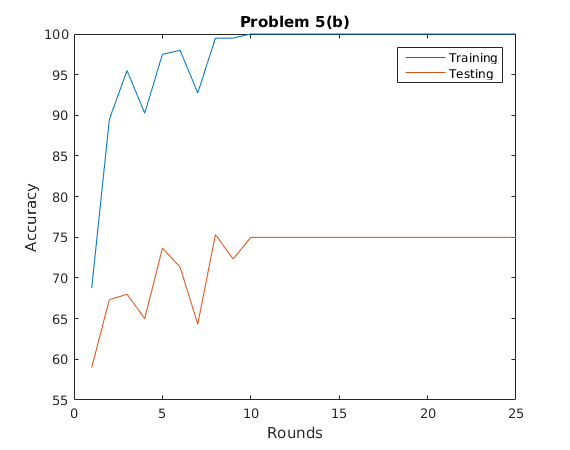
\includegraphics[scale=0.7]{../hw1_code_data/Problem5/plots/part-b/plot_5b.png}}
\end{figure}

\pagebreak
\subsubsection*{Part (c):}
$\eta$ value taken as 0.25.

\begin{figure}[H]
	\centering
	\fbox{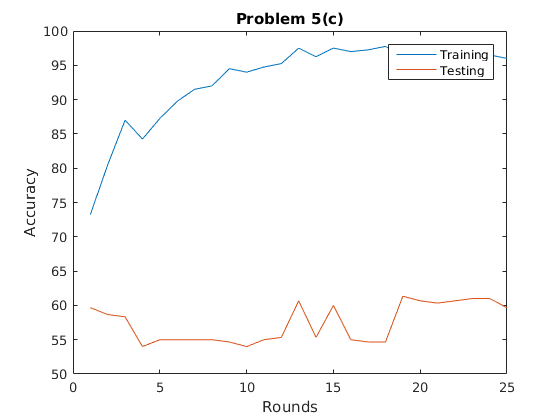
\includegraphics[scale=0.7]{../hw1_code_data/Problem5/plots/part-c/plot_5c.png}}
\end{figure}

\subsubsection*{Part (d):}
Top 10 influential features:
\begin{enumerate}
	\item titanic
	\item bad
	\item no
	\item they
	\item story
	\item nothing
	\item seagal
	\item would
	\item bit
	\item any
\end{enumerate}


\subsubsection*{Part (e):}
\begin{figure}[H]
	\centering
	\fbox{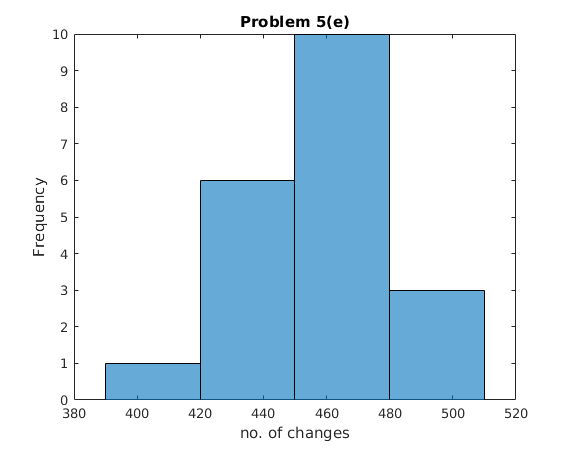
\includegraphics[scale=0.7]{../hw1_code_data/Problem5/plots/part-e/plot_5e.png}}
\end{figure}

\paragraph{}

We can see from the table below that there exist a positive value of $\gamma$ thus, the data is linearly separable. Also the upper bound from the following inequality is correct: 
$$\gamma \le  \frac{R^2 ||w||^2}{M}$$


\begin{center}
	\begin{tabular}{||c c||} 
		\hline
		Gamma & Gamma upper bound  \\ [0.5ex] 
		\hline\hline
		5 & 7.1022 e+07 \\
		\hline
		10 & 6.9681 e+07 \\
		\hline
		11 & 6.2964 e+07 \\
		\hline
		1 & 6.6023 e+07 \\
		\hline
		7 & 6.4864 e+07 \\
		\hline
		7 & 6.5349 e+07 \\
		\hline
		6 & 6.3785 e+07 \\
		\hline
		10 & 5.8274 e+07 \\
		\hline
		10 & 6.5096 e+07 \\
		\hline
		4 & 6.5724 e+07 \\
		\hline
		4 & 6.4086 e+07 \\
		\hline
		8 & 6.4305 e+07 \\
		\hline
		0 & 6.1728 e+07 \\
		\hline
		16 & 6.9228 e+07 \\
		\hline
		2 & 6.5416 e+07 \\
		\hline
		11 & 6.4969 e+07 \\
		\hline
		18 & 5.8436 e+07 \\
		\hline
		5 & 6.6827 e+07 \\
		\hline
		7 & 6.7941 e+07 \\
		\hline
		0 & 6.7997 e+07 \\
		\hline
		
		
	\end{tabular}
\end{center}



\subsubsection*{Part (f):}
\begin{center}
	\begin{tabular}{||c c c c||} 
		\hline
		$\eta$ & Updates & Training Acc. & Test Acc \\ [0.5ex] 
		\hline\hline
		0.05 & 416 & 100.0 & 75.0 \\
		\hline
		0.10 & 416 & 100.0 & 75.0 \\
		\hline
		0.15 & 460 & 100.0 & 75.0 \\
		\hline
		0.20 & 416 & 100.0 & 75.0 \\
		\hline
		0.25 & 416 & 100.0 & 75.0 \\
		\hline
		0.30 & 460 & 100.0 & 75.0 \\
		\hline
		0.35 & 460 & 100.0 & 75.0 \\
		\hline
		0.40 & 416 & 100.0 & 75.0 \\
		\hline
		0.45 & 416 & 100.0 & 75.0 \\
		\hline
		0.50 & 416 & 100.0 & 75.0 \\
		\hline
		0.55 & 432 & 100.0 & 71.3 \\
		\hline
		0.60 & 460 & 100.0 & 75.0 \\
		\hline
	\end{tabular}
\end{center}

\begin{figure}[H]
	\centering
	\fbox{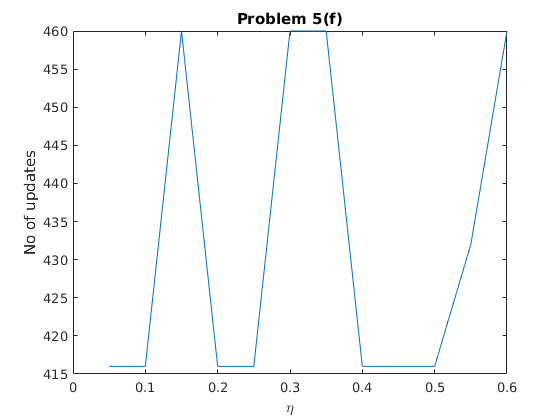
\includegraphics[scale=0.7]{../hw1_code_data/Problem5/plots/part-f/plot_5f.png}}
\end{figure}


\subsubsection*{Part (g):}

\begin{center}
	\begin{tabular}{||c c c ||} 
		\hline
		Dataset & Training Time & Test Accuracy \\ [0.5ex] 
		\hline\hline
		small & 0.4764  & 75.0 \\
		\hline
		medium & 0.8028 & 75.0 \\
		\hline
		large & 1.9427 & 75.3 \\
		\hline
	\end{tabular}
\end{center}

\paragraph{}
As can be seen from the graph below, the runtime complexity of perceptron increases linearly with the number of training examples. 



\begin{figure}[H]
	\centering
	\fbox{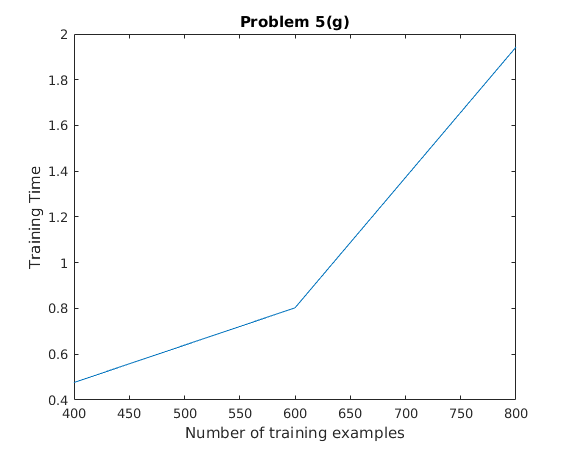
\includegraphics[scale=0.7]{../hw1_code_data/Problem5/plots/part-g/plot_5g.png}}
\end{figure}

\end{flushleft}
\end{document}


